\chapter{Robotics Applications}

This chapter will present the improvements of the Two-Layer teleoperation architecture developed within the i-Sur European project \cite{Ferraguti2015} for a needle insertion task.
First we present the teleoperation system modelled as a port-Hamiltonian system \cite{Ferraguti2015}, then we demonstrate both the equivalence between energy computation in task and joint space, and that a proper energy scaling between master and slave keeps the whole teleoperation system passive.
Finally we describe the two teleoperation schemas, a Position-Position and a Position-Force architecture. Both control architectures are endowed with \textit{pilot mode} for insertion assistance.

\section{A model for the teleoperation system}
The port Hamiltonian framework is a generalization of standard Hamiltonian mechanics, where energetic characteristics and power exchange between subsystems are clearly identified.
\subsection{The port-Hamiltonian description}
The most common representation of a port-Hamiltonian system is
\begin{equation}\label{General_Ham_system}
	\begin{cases}
		\dot{x} &= \left[ J(x)-R(x)\right] \dfrac{\partial H}{\partial x} + g(x)u\\
		y &= g^{T}(x)  \dfrac{\partial H}{\partial x}
	\end{cases}
\end{equation}
where $x \in \mathbb{R}^{n}$ is the state vector and $H(x): \ \mathbb{R}^{n} \rightarrow \mathbb{R}$ is the lower bounded Hamiltonian function representing the amount of energy stored in the system, $J(x) = -J(x)^{T}$ and $R(x) \geq 0$ are the matrices that represent the internal energetic interconnections and the dissipation of the port-Hamiltonian system, and $g(x)$ is the input matrix.
The input $u$ and output $y$ are dual variables and their product is (generalized) power.
The pair $(u^{T},y)$ represents the power exchanged by the system with the external world.
It can be shown that the following equality holds:
\begin{equation}
	\dot{H}(x) + \dfrac{\partial^{T} H}{\partial x}R(x) \dfrac{\partial H}{\partial x} = u^{T}(t)y(t)
\end{equation}
This means that the power supplied to the system is either stored or dissipated, thus that a port-Hamiltonian system is passive with respect to the pair $(u,y)$.\\
Let
\begin{equation}
	D(x) =  \dfrac{\partial^{T} H}{\partial x}R(x) \dfrac{\partial H}{\partial x} \geq 0
\end{equation}
be the power dissipated by the system. $D(x)$ represent the \textit{passivity margin}: the larger $D(x)$, the higher the passivity of the system.
A large passivity margin allows the system to absorb more energy generated by non passive actions while preserving its passivity.

\subsection{Port-Hamiltonian system with energy tank}\label{port_ham_system_with_tank}
The Two-Layer framework exploits the passivity margin by using of energy tank framework.
The energy dissipated by the system is stored in a (virtual) energy tank and can be used for implementing any desired control action in a passivity preserving way as described in Section \ref{Two-Layer-Approach}.\\
The model for a port-Hamiltonian system endowed with a tank is given by
\begin{equation}\label{Ham-Port-with-Tank}
		\begin{dcases}
	\dot{x} &= \left[ J(x)-R(x)\right] \dfrac{\partial H}{\partial x} + g(x)u\\
	\dot{x}_{t} &= \dfrac{\sigma}{x_{t}}D(x) + \dfrac{1}{x_{t}}(\sigma P_{in} - P_{out}) + u_{t}\\
	y_{1} &= 	\begin{pmatrix} y \\ \smallskip y_{t}\end{pmatrix}
	\end{dcases}
\end{equation}
where $x_{t}$ is the state associated with the energy storing tank, and 
\begin{equation}
	T(x_{t}) = \dfrac{1}{2}x^{2}_{t}
\end{equation}
is the energy stored in the tank.
$P_{in} \geq 0$ and $P_{out} \geq 0$ are the incoming and outgoing power flows that the tank can exchange with other tanks.
The pair $(u_{t}, y_{t})$ is the power port the tank can use to exchange energy with the external world and $y_{t} = \frac{\partial T}{\partial x_{t}} = x_{t}$. The parameter $\sigma \in \{0,1\}$ allows to upper bound the amount of energy stored in the tank.

The power balance for the tank is derived from the \eqref{Ham-Port-with-Tank}:
\begin{equation}\label{Tank-power-balance}
	\dot{T}=\sigma D(x) + \sigma P_{in} - P_{out} + u^{T}_{t}y_{t}
\end{equation}
which means that, if $\sigma = 1$, the tank stores the power dissipated by the system $D(x)$ and the incoming power flow $P_{in}$, while the outgoing power flow $P_{out}$ is released.
Furthermore the power can be injected and extracted from the tank via the power port $(u_{t}, y_{t})$.\\
In order to avoid singularities,($x_{t} = 0$ in \eqref{Ham-Port-with-Tank}) a small amount of energy must always be present in the tank, thus we chose an arbitrary small threshold $\varepsilon > 0$ representing the minimum amount of energy we want stored into it.
The tank has to be initialize and managed in such a way that $T(x_{0}) > \varepsilon$ and energy extraction is not allowed if $T(x_{0}) \leq \varepsilon$. It is also necessary to set the upper bound $\sigma$ mentioned before. In fact, if there is no bound, the energy available can become very large as time increases and it would be possible to implement behaviour that are unstable in practice, even if the system remain passive for a while.
Thus, $\sigma$ is set with the following policy:
\begin{equation}
	\sigma =
		\begin{dcases}
			1, \quad \mbox{if} \ T(x_{t}) \leq \bar{T}\\
			0, \quad \mbox{otherwise}
		\end{dcases}
\end{equation}
where $\bar{T}$ is an application dependent upper bound on the energy that can be stored in the tank.

The energy stored in the tank can be exploited for passively implementing any desired input $w \in \mathbb{R}^{n}$ to the port-Hamiltonian system with the tank is associated, by connecting the power port of the system $(u, y)$ with the power port of the tank $(u_{t}, y_{t})$ through the following preserving interconnection:
\begin{equation}\label{tank_power_preserving_interconnection}
	\begin{dcases}
		u &= \dfrac{w}{x_{t}}y_{t} = \dfrac{w}{x_{t}}x_{t} = w\\
		u_{t} &= \dfrac{-w^{t}}{x_{t}}y
 	\end{dcases}
\end{equation}
that implies the balance
\begin{equation}
	u^{T}y = -u^{T}_{t}y_{t}
\end{equation}
meaning that the energy supplied to/extracted from the port-Hamiltonian system for implementing the desired input is the same extracted from/supplied to the tank, consequently no energy is generated in the whole interconnected system.
\subsection{A port-Hamiltonian formulation for the tank-based teleoperation system }\label{sec:HamWithTank}
The master and slave manipulators in a teleoperation system not affected by communication delays can be represented with the formalism with $i=m,s$
\begin{equation}\label{teleop_Ham-Port-with-Tank}
	\left. 
	\begin{dcases}
		\begin{pmatrix}\dot{x_{i}} \\ \dot{p_{i}}\end{pmatrix}&= \begin{pmatrix} 0 & I \\-I & R_{i} \end{pmatrix} \begin{pmatrix} \dfrac{\partial H_{i}}{\partial x_{i}} \smallskip  \\ \dfrac{\partial H_{i}}{\partial p_{i}} \end{pmatrix} + \begin{pmatrix} 0\\ I\end{pmatrix}F_{ext,i} + \begin{pmatrix} 0 \\ I \end{pmatrix}F_{i}\\
		\dot{x}_{t_{i}} &= \dfrac{\sigma_{i}}{x_{t_{i}}}D_{i}(x) + \dfrac{1}{x_{t_{i}}}(\sigma \leftidx{^i}{P}{_{in}} -  \leftidx{^i}{P}{_{out}}) + u_{t_{i}}\\
		y_{i} &= 	\begin{pmatrix} v_{i} \\ \smallskip y_{t_{i}}\end{pmatrix}
	\end{dcases}
	\right. \qquad i=m,s
\end{equation}
where $x_{t_{i}}, y_{t_{i}} = x_{t_{i}}$, and $T_{i} = \frac{1}{2}x^{2}_{t_{i}}$ are the state of the tank, the output associated to the tank, and the energy stored in the tank respectively, $D_{i}$ represents the energy dissipated by the robot possibly increased by inserting a local damping injection (e.g. TLC) and $ \leftidx{^i}{P}{_{in}}$  and $\leftidx{^i}{P}{_{out}}$ are the power flows that can be exchanged with the tank. $F_{ext,i}$ are the external forces acting on the system and $F_{i}$ are the command provided by the passivity layer.\\
The coupling forces $F_{d,i} $ provided by the transparency layer are implemented using the energy available in the tanks by the following power preserving interconnection between the tank power port $(u_{t_{i}}, y_{t_i})$ and the robot power port $(F_{i}, v_{i})$:
\begin{equation}\label{robot-tank_interconnection}
	\left. 
	\begin{dcases}
		F_{i} &= \dfrac{F_{d,i}}{x_{t_{i}}}y_{t_{i}} = \dfrac{F_{d,i}}{x_{t_{i}}}x_{t_{i}} =F_{d,i}\\
		u_{t_{i}} &= -\dfrac{F^{T}_{d,i}}{x_{t_{i}}}v_{i} 
	\end{dcases}
	\right. \qquad i=m,s
\end{equation}
With this interconnection the command  $F_{d,i} $ provided by the transparency layer is implemented by exchanging energy with the tank: if $F_{d,i} >0$, it means that some amount of energy is necessary for implementing the desired input ans should be extracted from the tank. If $F_{d,i} <0 $, it means that the desired action is dissipative, thus the dissipated energy is stored in the tank.\\
The provided input could be passively achieved if and only if the tank is full enough, otherwise it could be either modulated by some passivation strategy or completely  cut off as explained in Section \ref{Two-Layer-Approach}.

If the tank goes below the threshold $T({x_{t_{i}}}) \leq \varepsilon_{i}$, energy extraction is forbidden and the coupling force implemented is $F_{d,i} = 0$.
This ensure the passivity and a stable behaviour of the teleoperation system but, it negatively affects its transparency.\\
It is then necessary to ensure that, both at the master and slave side, the level of the tank is kept much higher than a more conservative minimum level.
There are two methods for increasing the local tank level: transfer energy from the remote tank and extract it from the local robot by damping injection (TLC). The former should be preferred over the latter as it does not affect the dynamic of the system and does not affect either the feedback perceived by the user, as well.\\
The energy transfer strategy acts as follows: when the energy is below the more conservative minimum threshold $\leftidx{^i}{T}{_{req}}$, an \textit{energy quantum} is requested from the other tank. If at the other side the fill level of the tank is high enough, namely it is greater than a threshold $\leftidx{^i}{T}{_{ava}}$, an \textit{energy quantum} is sent. This \textit{availability} threshold helps to keep the energy balanced through the two sides.
Furthermore, if the tank is already full, all the energy dissipated by the local robot is sent to the other side in order to recover it.
Formally the request signal is:
\begin{equation}
	\left. 
	\leftidx{^i}{E}{_{req}}=
	\begin{dcases}
		1, \quad & \mbox{if} \ T_{i}(x_{t_{i}}) < \leftidx{^i}{T}{_{req}}\\
		0, \quad & \mbox{otherwise} 
	\end{dcases}
	\right. \qquad i=m,s
\end{equation}
and the whole energy transfer strategy could be described as
\begin{equation}\label{Transmission_strategy}
	\left\lbrace 
	\begin{aligned}
		\leftidx{^m}{P}{_{out}} &=(1- \sigma_{m})D_{m} + 	\leftidx{^s}{E}{_{req}} \beta_{m}\bar{P}_{m} =  \leftidx{^s}{P}{_{in}} \\
		\leftidx{^s}{P}{_{out}} &= (1- \sigma_{s})D_{s} + 	\leftidx{^m}{E}{_{req}} \beta_{s}\bar{P}_{s} =  \leftidx{^m}{P}{_{in}}
	\end{aligned}
	\right.
\end{equation}
where, as discussed in Section \ref{port_ham_system_with_tank}, if the tank is already full we send to the other tank the energy dissipated by the robot setting $\sigma_{i} = 0$.\\
The variable $\beta_{i} \in \lbrace 0, 1 \rbrace$ enables/disables the transfer of the energy from the tank, and its value is given by
\begin{equation}
	\left.
	\beta_{i} =
	\begin{dcases}
		1, \quad & \mbox{if} \ T_{i}(x_{t_{i}}) \geq \leftidx{^i}{T}{_{ava}}\\
		0, \quad & \mbox{otherwise}.
		\end{dcases}
	\right.
\end{equation}
$\bar{P_{i}} > 0$ is the rate of energy flowing from one tank to the other and it's a design parameter. The bigger $\bar{P_{i}}$ , the faster the energy transfer.\\
All  these thresholds are also application dependent, and the following constrain must be satisfied: $\varepsilon_{i} < \leftidx{^i}{T}{_{req}} < \leftidx{^i}{T}{_{ava}} < \bar{T}_{i}$ , for $i=m,s$\\

This teleoperation schema is passive with respect to the environment, i.e. it is passive with respect to the pair $\left(\left(F^{T}_{h} , F^{T}_{e}\right)^T, \left( v^{T}_{m}, v^{T}_{s}\right)^{T} \right)$ 
\begin{proof} \cite{Ferraguti2015}
	Consider the total energy of the teleoperation system as a storage function:
	\begin{equation}
		H(t) = H_{m}(t) + H_{s}(t) + T_{m}(t) + T_{s}(t)
	\end{equation}
	Using \eqref{teleop_Ham-Port-with-Tank} we obtain that
	\begin{equation}\label{energy_balance_teleop_Ham-Port-with-Tank}
		\begin{split}
		\dot{H}(t) = &-D_{m}(t) + F^{T}_{m}v_{m}  +\sigma_{m}D_{m}(t) +\sigma_{m} \leftidx{^m}{P}{_{in}} - \leftidx{^m}{P}{_{out}}\\ 
		&-D_{s}(t) +  F^{T}_{s}v_{s} +\sigma_{s}D_{s}(t) +\sigma_{s} \leftidx{^s}{P}{_{in}} - \leftidx{^s}{P}{_{out}} \\
		& +u_{t_{m}}y_{t_{m}} + F^{T}_{h}v_{m} +u_{t_{s}}y_{t_{s}} + F^{T}_{e}v_{s}
		\end{split}
	\end{equation}	
	Since the tanks and the robots are interconnected with the power preserving interconnection \eqref{robot-tank_interconnection}, we have that $F^{T}_{i}v_{i} = -u_{t_{i}}y_{t_{i}} $, where $i=m,s$ thus the \eqref{energy_balance_teleop_Ham-Port-with-Tank} can be rewritten as
	\begin{equation}
		\begin{split}
			\dot{H}(t) = & -(1 - \sigma_{m})D_{m}(t) - (1 - \sigma_{s})D_{s}(t)\\
									& -(1 - \sigma_{m}) \leftidx{^m}{P}{_{in}} -(1 - \sigma_{s}) \leftidx{^s}{P}{_{in}} \\
									& + F^{T}_{h}v_{m} + F^{T}_{e}v_{s}
		\end{split}
	\end{equation}
	Finally using \eqref{Transmission_strategy}, we have that
	\begin{equation}
	\begin{split}
			\dot{H}(t) = & -(1 - \sigma_{m})D_{m}(t) - (1 - \sigma_{s})D_{s}(t)\\
			& -(1 - \sigma_{m}) \leftidx{^s}{P}{_{out}} -(1 - \sigma_{s}) \leftidx{^m}{P}{_{out}} \\
			& + F^{T}_{h}v_{m} + F^{T}_{e}v_{s}
		\end{split}
	\end{equation}
	and since $\sigma_{i} \in \{0,1\}$, $\leftidx{^i}{P}{_{out}}$, $D_{i} \geq 0$ for $i=m,s$ it follows that
	\begin{equation}
		\dot{H}(t) \leq F^{T}_{h}v_{m} + F^{T}_{e}v_{s}
	\end{equation}
thus \eqref{Two_layer_passivity_world} holds, which proves our statement.
\end{proof}
Augmenting the local damping, via the TLC approach, is a passivity preserving technique. For a formal proof the port-Hamiltonian model should be rewritten with a variable damping matrix and the previous proof is similar.

%%%%%%%%%%%%%%%%%%%%%%%%%%%%%%%%%%%%%%%%%%%%%%%%%%%
\section{Improvements  on the Two-Layer  }\label{TwoLayer_improvements}
The Two Layer approach is a really versatile and powerful tool for the development of a passive bilateral teleoperation system. Although there is some space to exploit it, giving even more flexibility and control to the designer in order to better manage transparency, thus preserving passivity, even neglecting the dynamic model of the two manipulators involved.
%%TODO esprimiti o cancella.

\subsection{Energy evaluation in task space}
Both in the i-Sur project and in the original paper from Frankel \textit{et. all} \cite{Franken2011}, energy computation and the passification strategy are performed in the joint space.
For a single DoF device it is less challenging to develop a passification strategy and analyse how the transparency of the system is affected. But for a multi DoF device the passification strategy could heavily affect transparency: a uniform action between the joints could, due to the kinematics mapping, results in a dangerous behaviour in the task space.\\
Take needle insertion as an example: for ensuring the safety of the patient, when no needle steering techniques are involved,  the path executed must follow the needle's main $z$ axis.
It is desirable that also the passivity strategy could, in a way, act preserving, as much as possible, transparency in the task space to ensure the patient safety. In this example could be a good idea splitting the task into two subtasks with different degrees of transparency priority.\\
An high degree of priority task should ensure the correct $x-y$ position and orientation of the needle tip, the other one, which could afford more safely a lower degree of transparency, performs the puncturing action along the $z$ axis.
In fact if there is not enough energy for performing the full action, the system will puncture with less force but the needle will not injure neighbour tissues.\\
This approach requires only minimal changes into the passivity layer: in fact the notion of transparency affects only the strategy on how $\tau_{max}$ is computed in \eqref{tau_TL}.
The development of a task-oriented passivity approach requires energy evaluation in the task space.
Furthermore, this approach for energy evaluation allows the designer to work in a well known spatial domain, thus better understand the behaviour of the system, where to act and how to tune the parameters of the system to achieve a more stable behaviour. 

\begin{theorem}\label{Energy_equivalence}
	\emph{\textbf{Energy equivalence between joint and task space}}\\
	The amount of energy required in task space to perform a task is equal to the one in joint space.
\end{theorem}
The proof of this statement requires the notion of Jacobian and  Static Wrench Transmission.\\
The Jacobian matrix $J(q)$ allows the solution to the forward instantaneous kinematics problem for a serial chain manipulator, where the total velocity of the end effector has to be found given the  the position and velocitiy of all members of the chain joints
\begin{equation}\label{Jacobian}
	\leftidx{^k}{v}{_{N}} = J(q)\dot{q}
\end{equation}
where $\leftidx{^k}{v}{_{N}}$ is the spatial velocity of the end effector expressed in the frame $k$, $\dot{q}(t)$ the $n$-dimensional vector composed of the joints rates and $J(q)$ is a $6 \times n$ matrix whose elements are, in general, non-linear function of $q$ and is expressed relative to the same coordinate frame as the spatial velocity $\leftidx{^k}{v}{_{N}}$ \cite{Siciliano:2007:SHR:1209344}.\\
The static wrench transmission establishes the relationship between wrenches applied to the end effector and forces/torques applied to the joints.
Exploiting the principle of virtual work, the relationship between wrenches applied to the end effector and force/torques applied to the joints can be shown to be
\begin{equation}\label{jForce}
	\tau = J^{T} f
\end{equation}			
where $\tau$ is the $n$-dimensional vector of applied joint forces/torques for an $n$-Dof manipulator and $f$ is the spatial wrench vector
\begin{equation}
f =  \begin{bmatrix}
\mathrm{f}\\ o
\end{bmatrix}
\end{equation}				
in which $o$ and $\mathrm{f}$ are the vectors of torques and forces, respectively, applied to the end-effector, both expressed in the coordinate frame where the Jacobian is expressed. The Jacobian maps the joint rates into the spatial velocity of the end-effector, its transpose maps the wrenches applied into the end-effector into joint forces/torques \cite{Siciliano:2007:SHR:1209344}.
The formalization for Theorem \ref{Energy_equivalence} is:
\begin{equation}
E = \int \tau^{T}(t)\dot{q}(t)dt = \int f^{T}(t)\dot{x}(t)dt
\end{equation}
and can be proved as follows
\begin{proof}
Consider the formulation of energy in joint space
\begin{equation}
	E_{\tau} = \int \tau^{T}(t)\dot{q}(t)dt
\end{equation}
thus we can write the elementary work in joint space as
\begin{equation}
	dW_{\tau} = \tau^{T}(t) dq \quad \text{.}
\end{equation}
The energy in task space is
\begin{equation}
E_{\mathrm{f}} = \int f^{T}(t)\dot{x}(t)dt
\end{equation}
and the elementary work in task space is
\begin{equation}
	dW_{\mathrm{f}} = f^{T}(t)dx \quad \text{.}
\end{equation}
Using \eqref{Jacobian} we end up will
\begin{equation}\label{force_cart_velocity as joint}
	dW_{f} = f^{T}(t)J(q)dq
\end{equation}
Manipulators are time independent system with holonomic constraints: their pose depends only on joints positions, meaning that virtual displacements match physicals ones.\\
By this consideration we can write
\begin{equation}
	\delta W_{\tau} = \tau^{T}(t) \delta q
\end{equation}
\begin{equation}
	\delta W_{ f}=f^{T}(t)J(q) \delta q
\end{equation}
and for the principle of virtual works
\begin{equation}
	\delta W_{\mathrm{f}} =\delta W_{\tau} \quad \forall \delta q
\end{equation}
Now using \eqref{jForce} in \eqref{force_cart_velocity as joint}
\begin{equation}
	\begin{split}
	dW_{ \mathrm{f}} &= \mathrm{f}^{T}(t)J(q)dq\\
	&=\tau^{T}(t)J^{T}(q)J(q)dq\\
	&=\tau^{T}(t)dq\\
	&= dW_{\tau} 			
 	\end{split}
\end{equation}
\end{proof}
For a redundant manipulator in \eqref{jForce} the Jacobian pseudoinverse has to be addressed instead of $J^{T}$.
\subsection{Energy scaling}
When dealing with a pair of the similes manipulator, jointly coupled, performing the commanded task at the slave side will require the same amount of energy supplied at the master side.
This is not true when dealing with manipulators that are mechanically different.
Performing the same task require different amount of energy, even if the Cartesian motion is exactly the same.
This is due to the different dynamical model of the two manipulators. Furthermore manipulator friction is another energy dissipative unknown variable to deal with.
When adopting an energy based approach for enforcing the passivity of the interconnected teleoperation system, all these effects produce an energy leakage.

%%%%%%%%%%%%%%
With the purpose to balance the different energy requirement between the two manipulators, we introduce a couple of constants $\alpha$ and $\gamma$ such that
\begin{equation}\label{Scaling_condition}
	\alpha \gamma = 1 \qquad \alpha,\gamma >0
\end{equation}
When performing the energy transmission between the two tanks, the master, which have a low inertia, send to the slave, which have a greater inertia, a properly scaled up quantum of energy to compensate the energy requirement between the two manipulator. The slave do the same but scaling down the value of the quantum of energy.
In other words, if we set in e.g. $\alpha = 10$, then $\gamma = \frac{1}{10}$, it means that an action performed on the master requires ten times more energy to be replicated on the slave, at the same time a feedback from the slave require one tenth of the original energy to be executed on the master.\\
This idea clearly affects the energy transmission strategy that, with the introduction of energy scaling, becomes
\begin{equation}\label{Transmission_strategy_scaled}
	\left\lbrace 
	\begin{aligned}
		\alpha \leftidx{^m}{P}{_{out}} &= \alpha \left( (1- \sigma_{m})D_{m} + 	\leftidx{^s}{E}{_{req}} \beta_{m}\bar{P}_{m} \right) = \leftidx{^s}{P}{_{in}} \\
	\gamma	\leftidx{^s}{P}{_{out}} &= \gamma \left( (1- \sigma_{s})D_{s} + 	\leftidx{^m}{E}{_{req}} \beta_{s}\bar{P}_{s}\right)  = \leftidx{^m}{P}{_{in}}
	\end{aligned}
	\right.
\end{equation}
This enhancement preserves the passivity of the whole teleoperation system.
%%%%%%%%%%%%%%
The proof can be shown looking at the whole architecture either from the master, or from the slave side.
Interdependently of the choice, each side sees the energy at the other side proportionally scaled by its scale factor.
\begin{proof}\textbf{Slave side}\\
Let focus on the slave side. The storage function that represent the energy in the system is
	\begin{equation}\label{slave_scaled_storage_function}
		\hat{H}_{s}(t) = \alpha H_{m}(t) + H_{s}(t) + \alpha T_{m}(t) + T_{s}(t)
	\end{equation}
	Using \eqref{teleop_Ham-Port-with-Tank} we obtain that
	\begin{equation}
		\begin{split}
		\dot{\hat{H}}_{s}(t)= & -\alpha D_{m}(t) + \alpha F^{T}_{m}v_{m}  +\sigma_{m}\alpha D_{m}(t) + \alpha\left( \sigma_{m} \leftidx{^m}{P}{_{in}} - \leftidx{^m}{P}{_{out}}\right)\\ 
		& -D_{s}(t) +  F^{T}_{s}v_{s} +\sigma_{s}D_{s}(t) + \left( \sigma_{s} \leftidx{^s}{P}{_{in}} - \leftidx{^s}{P}{_{out}}\right)\\
		& + \alpha u_{t_{m}}y_{t_{m}} + \alpha F^{T}_{h}v_{m} +u_{t_{s}}y_{t_{s}} + F^{T}_{e}v_{s}
		\end{split}
	\end{equation}	
	Since the tanks and the robots are interconnected with the power preserving interconnection \eqref{robot-tank_interconnection}, we have that $F^{T}_{i}v_{i} = -u_{t_{i}}y_{t_{i}} $, where $i=m,s$.\\
	Substituting \eqref{Transmission_strategy_scaled} we have
	\begin{equation}
		\begin{split}
			\dot{\hat{H}}_{s}(t) = & -(1 - \sigma_{m})\alpha D_{m}(t) - (1 - \sigma_{s})D_{s}(t)\\
			& \sigma_{m} \alpha \gamma \leftidx{^s}{P}{_{out}} - \leftidx{^s}{P}{_{out}} + \sigma_{s} \alpha \leftidx{^m}{P}{_{out}} - \alpha \leftidx{^m}{P}{_{out}}\\
			& + \alpha F^{T}_{h}v_{m} + F^{T}_{e}v_{s}
		\end{split}
	\end{equation}
	Rearranging terms, we end up with
	\begin{equation}
		\begin{split}
			\dot{\hat{H}}^{s}(t) = & -(1 - \sigma_{m})D_{m}(t) - (1 - \sigma_{s})D_{s}(t)\\
			& -(1 - \sigma_{m}) \leftidx{^s}{P}{_{out}} -(1 - \sigma_{s}) \alpha \leftidx{^m}{P}{_{out}} \\
			& + \alpha F^{T}_{h}v_{m} + F^{T}_{e}v_{s}
		\end{split}
	\end{equation}
	and since $\sigma_{i} \in \{0,1\}$, $\leftidx{^i}{P}{_{out}}$, $D_{i} \geq 0$ for $i=m,s$ it follows that
	\begin{equation}
			\dot{\hat{H}}_{s}(t) \leq \alpha F^{T}_{h}v_{m} + F^{T}_{e}v_{s} \quad \text{.}
	\end{equation}
	Thus \eqref{Two_layer_passivity_world} holds, which proves our statement.
\end{proof}
The same could be done from the master point of view by considering the storage function $\hat{H}_{m}(t)$
	\begin{equation}
\hat{H}_{m}(t) = H_{m}(t) + \gamma H_{s}(t) + T_{m}(t) + \gamma T_{s}(t)
\end{equation}
instead of \eqref{slave_scaled_storage_function}.
\section{Implemented teleoperation schemes}
The effectiveness of this approach has been evaluated with two different control schemes implemented within the transparency level: a position-position (PP), for bilateral motion synchronism and a position-force (PF) for better force reflection. 
\subsection{Position - Position (P-P)}\label{PP_architecture}
\begin{figure}
	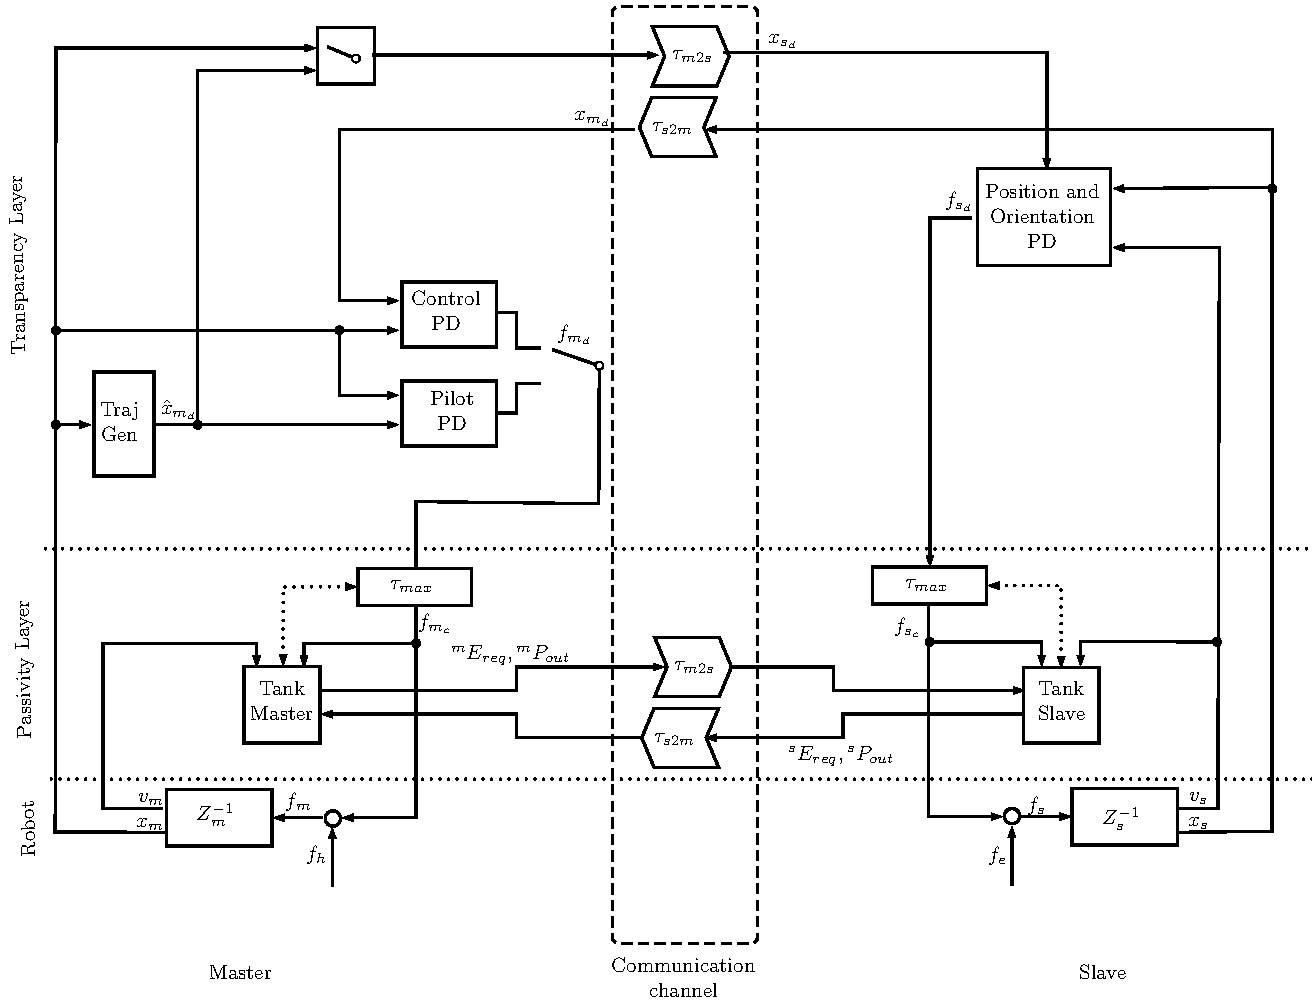
\includegraphics[width=\linewidth]{schemas/TwoLayerPPok.pdf}
	\caption[The implemented P-P architecture]{The implemented position-position architecture}
	\label{sch:TwoLayerPP}
\end{figure}
As shown in \figurename{ \ref{sch:TwoLayerPP}}, the first teleoperation schema implemented in the transparency layer is a simple Position-Position.
The main goal of such schema is to achieve a synchronism between the two manipulator poses.\\
Master pose is sent to the slave on which a PD controller is in charge of tracking the commanded Cartesian position and orientation.
Slave pose is sent back to the master and used as a feedback signal that tells the operator if the slave robot is moving in free space or if it is in contact with the environment. This is possible thanks to the virtual spring-damper coupling operated by the PD controller.
In fact the virtual displacement between the two manipulator produces a force acting at both side.\\
When the slave is in free motion, at master side the error between the desired pose, imposed by the operator, and the feedback one is small. The slave can freely follow the pose commanded by the master, reducing the tracking error. The operator feels this little tracking displacement as a sort of inertia.\\
When the slave is in contact, the tracking displacement increases. At master side the error between the desired pose and the feedback one also increases, providing a stronger reaction force that acts as a kinaesthetic feedback.\\
Because of the P-P architecture the error displacement is the same at both sides, thus the kinaesthetic feedback induced at master side is mainly proportional to the force being applied at master side through the relationship between $K_{p_{master}} $ and $K_{p_{slave}}$.
The remaining force is due to the presence of a damping factor $K_{d}$ acting on the error derivative.

The slave PD pose controller is made by two separate PD controllers that works in parallel.
The former acts on the Cartesian position and performs a linear control on the position error in task space. Its outputs are the control Cartesian forces, expressed in the slave's base frame, commanded to the robot.\\
The position error in task space is
\begin{equation}
e_{pos} = \left( x_{pos_{d}}-  x_{pos}\right) 
\end{equation}
where $x_{pos_{d}}$ is the vector of Cartesian position commanded by the master and  $x_{pos}$ the vector of current slave position\\
The position PD controller is formulated as
\begin{equation}
	\mathrm{f}(t)= K_{p_{pos}}e_{pos}(t) + K_{d_{pos}}\dfrac{de_{pos}(t)}{dt}
\end{equation}
where $K_{p_{pos}}$ and $K_{d_{pos}}$ are $3\times3$ diagonal matrices of the position control gains.
The latter acts on Cartesian orientation and performs a linear control action on the orientation error in task space. Its output are the control Cartesian torques, expressed in the slave's base frame, commanded to the robot.
The orientation error in task space is
\begin{equation}
e_{ang} = \left( x_{ang_{d}} -  x_{ang}\right) 
\end{equation}
where $x_{ang_{d}}$ and  $x_{ang}$ are the Cartesian orientation commanded by the master and the current slave orientation respectively.\\
The orientation PD controller is formulated as
\begin{equation}
o = K_{p_{ang}}e_{ang}(t) + K_{d_{ang}}v_{ang}(t)
\end{equation}
where $K_{p_{ang}}$ and $K_{d_{ang}}$ are $3\times3$ diagonal matrices of the position control gains, and $v_{ang}(t)$ is the slave's Cartesian angular velocity vector.
The stronger damping action on the orientation controller helps the system stability.\\
The two components of the Cartesian wrench command, forces $\mathrm{f}$ and torques $o$ are then passivated by the passivity layer ($\tau_{max}$) and then mapped into joints torque through the Jacobian Pseudo-inverse.
This mapping is performed by the robot itself.

At master side, when performing the standard bilateral P-P teleoperation, acts the same PD controller presented for the slave, tuned with proper values for $K_{p_{pos}}$, $K_{d_{pos}}$, $K_{p_{ang}}$ and $K_{d_{ang}}$.

Before performing the puncturing, the clinician could switch from this controller to a specialized one, previously mentioned as \textit{pilot mode}, designed to help the operator to perform a more precise puncture along the needle's $z$ axis direction.\\
A trajectory generator holds the values of the master orientation and $x-y$ position relative to the end-effector reference frame at switching time. The z position, instead, is always the current one.\\
This new conditioned command, $\hat{x}$, is provided both as a reference for the slave and as a reference value for the local PD controller.\\
In order to provide a different kind of feedback when in this mode, the PD controller is replicated thus we could use different gains.\\
The operator feels a constrain force that guides him moving only along $z$, in this direction the coupling between the master and the slave is preserved together with the feedback.\\
This controller switching ability is clearly a non passive solution. However we can safely apply such strategy because of the Two-Layer architecture guarantees the passivity of the system.

%The positional portion of the PD (Proportional, Derivative) is the classical, well established in control theory, controller operating on the error between the reference and current signal.
%The orientational ones, operates proportionally on the position error but the derivative gain acts on the full current velocity signal, providing a stronger damping action.
%
%The output of the controller are the two components of the control twist expressed into the robot base frame: respectively cartesian forces and torques.
%
%This command is passivated by the passivity layer ($\tau_{max}$) and then mapped as joints torque trough the Jacobian Pseudo-inverse.
%
%$K_{p_{lin}}, K_{d_{lin}}, K_{p_{ang}}, K_{d_{ang}}$ are arbitrary chosen, application dependant, diagonal matrices 3x3 of the control gains.
%
%When performing the puncturing the clinician could switch to specialized controller at the master side: at transition time, the trajectory generator fixes the current orientation, and the relative x,y position of the end effector.
%This fixed pose is also sent to the slave in order to improve the accuracy. The only free variable in the system is the linear z axes which means that at slave side we can move only along the shaft of the needle.
%The operators feels a force that acts as a virtual set of springs that allows free movement only along master z axis. With the purpose of providing the puncturing feedback the slave's feedback signal acts only on the z axes.
%
%This controller switching ability is clearly a non passive solution, thus we can safely apply such strategy because of the two layer guarantees on the passivity of the system.
%
\subsection{Position - Force (P-F)}\label{sec:position---force-p-f}
\begin{figure}
	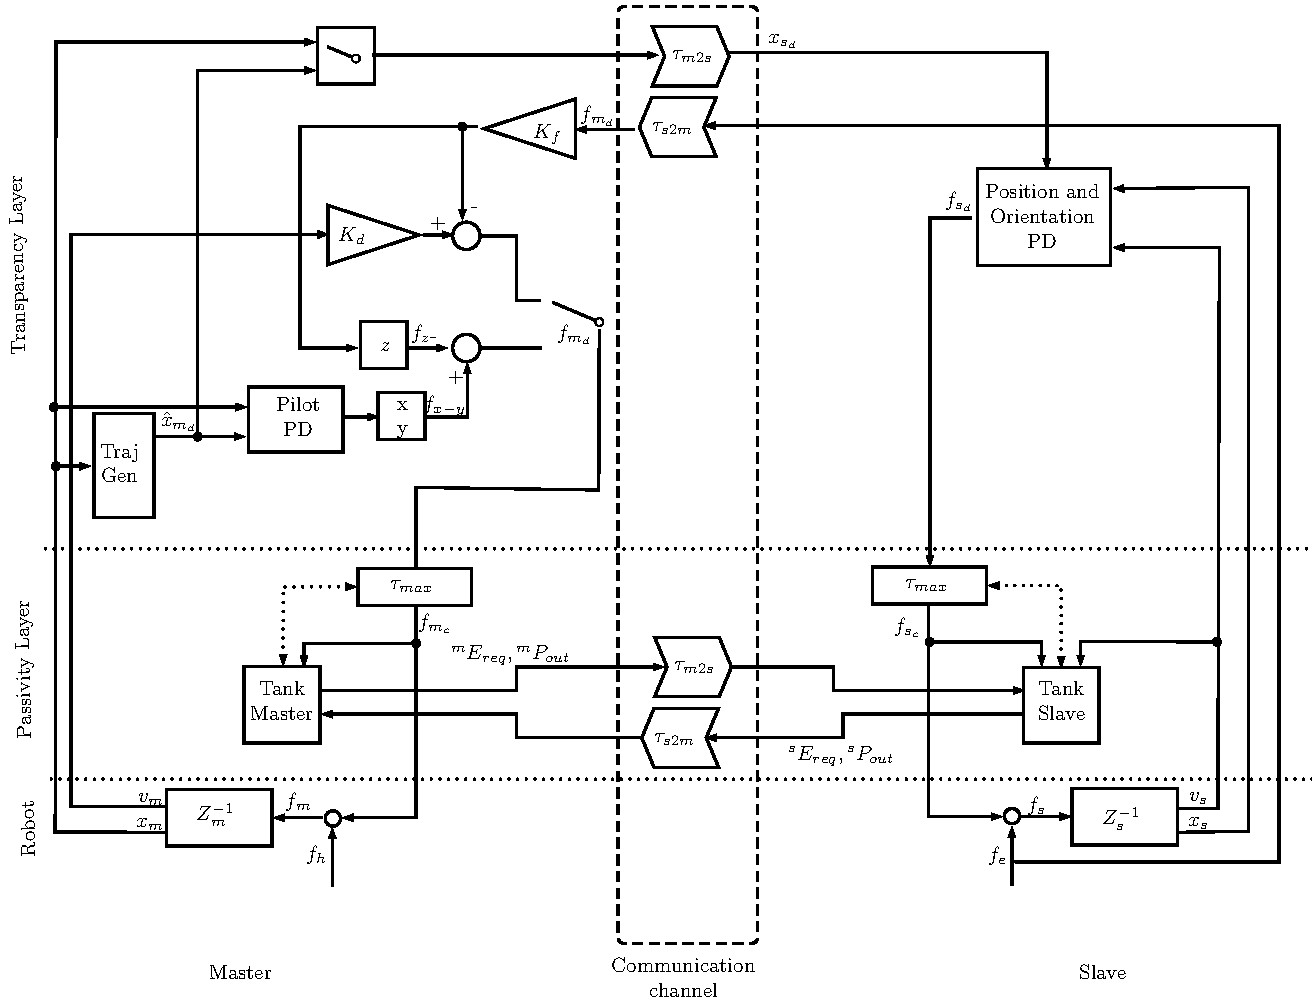
\includegraphics[width=\linewidth]{schemas/TwoLayerPFok.pdf}
	\caption[The implemented P-F architecture]{The implemented position-force architecture}
	\label{sch:TwoLayerPF}
\end{figure}

The latter teleoperation scheme implemented is a simple Position-Force, an illustration is available in \figurename{ \ref{sch:TwoLayerPF}}, 
The main goal of such scheme is providing a more effective force feedback to the operator.

Master pose is sent to the slave on which, the same PD controller of the previous scheme is in charge to track the commanded Cartesian position and orientation.
The feedback signal $f_{slave}$ from the slave is the interaction wrench provided by a force sensor.
At the master side this signal could be scaled down by the $K_{f}$ gain which is, again, a $6\times6$ diagonal matrix of gains.\\
Because of the two layer algorithm, we have to produce some amount of energy to perform actions at slave side while in free motion (if there are no interaction forces, the commanded force on the master is null and consequently the instantaneous power is zero).
This is achieved introducing a small and constant damping.
The wrench applied to the master and thus perceived by the operator is
\begin{equation}
		\mathrm{f}(t) = K_{f}f_{slave}(t) - K_{d} v_{m}(t)
\end{equation}
where $K_{d}$ is a $6\times6$ diagonal matrix of damping gains and $v_{m}$ is the master velocity.

Even in this architecture, the clinician before performing the puncturing could switch to the specialized controller.
The purpose is the same from the P-P architecture: provide a tool to help the operator to perform a more precise puncture along the needle's $z$ axis direction.\\
To achieve this goal the \textit{pilot mode} for this schema is a hybrid position-force controller.
It acts as PD controller for orientation and for the position along $x-y$ axes while keeping the original slave force feedback along $z$.\\
The trajectory generator holds the values of the master orientation and $x-y$ position relative to the end-effector frame of reference at switching time.
This conditioned signal, $\hat{x}$, is provided both as a reference for the slave and as reference value for the local PD controller. 
The operator feels a constrain force that forces him moving only along the master tool $z$ axis, in this direction the operator feels the corresponding force feedback from $f_{slave}$ modulated trough $K_{f}$ gain.
This controller switching ability is clearly a non passive solution. However we can safely apply such strategy because of the Two-Layer architecture guarantees the passivity of the system.

\section{Discussion}
In this chapter with the Two-Layer teleoperation architecture modelled as a port-Hamiltonian system,
we showed that energy evaluation is equivalent in task and in joint space.
A proper energy scaling strategy has been proposed to allow the coupling, in a passive way, of very different manipulators.
Finally we described the two teleoperation schemas implemented upon this formulation of Two-Layer algorithm.


%%%%%%%%%%%%%%%%%%%%%
\clearpage
\thispagestyle{empty}